%%%%%%%%%%%%%%%%%%%%%%%%%%%%%%%%%%%%%%%%%
% a0poster Portrait Poster
% LaTeX Template
% Version 1.0 (22/06/13)
%
% The a0poster class was created by:
% Gerlinde Kettl and Matthias Weiser (tex@kettl.de)
%
% This template has been downloaded from:
% http://www.LaTeXTemplates.com
%
% License:
% CC BY-NC-SA 3.0 (http://creativecommons.org/licenses/by-nc-sa/3.0/)
%
%%%%%%%%%%%%%%%%%%%%%%%%%%%%%%%%%%%%%%%%%

%----------------------------------------------------------------------------------------
%	PACKAGES AND OTHER DOCUMENT CONFIGURATIONS
%----------------------------------------------------------------------------------------

\documentclass[a0,portrait]{a0poster}

\usepackage{multicol} % This is so we can have multiple columns of text side-by-side
\columnsep=100pt % This is the amount of white space between the columns in the poster
\columnseprule=3pt % This is the thickness of the black line between the columns in the poster

\usepackage[svgnames]{xcolor} % Specify colors by their 'svgnames', for a full list of all colors available see here: http://www.latextemplates.com/svgnames-colors

\usepackage{times} % Use the times font
%\usepackage{palatino} % Uncomment to use the Palatino font

\usepackage{subfig}
\usepackage{graphicx} % Required for including images
\graphicspath{{figures/}} % Location of the graphics files
\usepackage{booktabs} % Top and bottom rules for table
\usepackage[font=small,labelfont=bf]{caption} % Required for specifying captions to tables and figures
\usepackage{amsfonts, amsmath, amsthm, amssymb} % For math fonts, symbols and environments
\usepackage{wrapfig} % Allows wrapping text around tables and figures
\usepackage{polyglossia}
    \setdefaultlanguage{portuges}
\usepackage{microtype}
\usepackage{verbatim}
\usepackage{ragged2e}
\usepackage{framed}
\usepackage{hyperref}
\usepackage{url}
%\usepackage{showframe}

\begin{document}

\frenchspacing

%----------------------------------------------------------------------------------------
%	POSTER HEADER
%----------------------------------------------------------------------------------------

% The header is divided into two boxes:
% The first is 75% wide and houses the title, subtitle, names, university/organization and contact information
% The second is 25% wide and houses a logo for your university/organization or a photo of you
% The widths of these boxes can be easily edited to accommodate your content as you see fit

\begin{minipage}[b]{0.75\linewidth}
\veryHuge \color{NavyBlue} \textbf{Aprendizado de Máquina em Textos} \color{Black}\\ % Title
\Huge\textit{Identificando Idiomas com \emph{Machine Learning}}\\[2cm]
\huge \textbf{Jorge Ashkar Ferreira Simondi --- 8517081,\\
              Leonardo de Almeida Lima Zanguetin --- 8531866,\\
              Victor Luiz da Silva Mariano Pereira --- 8602444}\\[1cm]
%\huge Instituto de Ciências Matemáticas e de Computação -- ICMC\\
%\huge Universidade de São Paulo -- USP
\end{minipage}
%
\begin{minipage}[b]{0.25\linewidth}

\includegraphics[width=17cm]{LOGO_ICMC_CMYK.png}

\includegraphics[width=8cm]{brasao_usp1.png}
\end{minipage}

\vspace{1cm} % A bit of extra whitespace between the header and poster content

%----------------------------------------------------------------------------------------

\begin{multicols}{2} % This is how many columns your poster will be broken into, a portrait poster is generally split into 2 columns

\begin{abstract}
    Reconhecer em qual idioma um texto está escrito, hoje em dia, é algo de suma importância. Apesar de ter várias ferramentas prontas na internet, nesse trabalho, mostraremos uma forma de como aplicar inteligência artificial para fazer essa classificação. Uma visão desde a análise dos dados até o treinamento para o aprendizado de máquina.
\end{abstract}

%----------------------------------------------------------------------------------------
%	INTRODUCTION
%----------------------------------------------------------------------------------------

\section*{Introdução}
A análise de textos em línguas diferentes pode ser feita de diversas maneiras, uma delas é em relação as palavras, a qual temos que verificar em qual dicionário está. Porém, uma outra forma de analisar é pela frequência de cada caractere, e essa é a abordagem que usaremos.

\begin{multicols}{2}
    \begin{framed}
        \texttt{Perceived end knowledge certainly day sweetness why cordially. Ask quick six seven offer see among. Handsome met debating sir dwelling age material. As style lived he worse dried. Offered related so visitor we private removed. Moderate do subjects to distance.\\Of friendship on inhabiting diminution discovered as. Did friendly eat breeding building few nor. Object he barton no effect played valley afford. Period so to oppose we little seeing or branch. Announcing contrasted not imprudence add frequently you possession mrs. Period saw his houses square and misery.}
    \end{framed}
    \captionof{figure}{Texto do Random Text Generator~\cite{site:rtg}}
    \begin{framed}
        \texttt{Ainda assim, existem dúvidas a respeito de como a execução dos pontos do programa facilita a criação das direções preferenciais no sentido do progresso. Por outro lado, o novo modelo estrutural aqui preconizado cumpre um papel essencial na formulação das novas proposições.\\O empenho em analisar o consenso sobre a necessidade de qualificação exige a precisão e a definição dos relacionamentos verticais entre as hierarquias. Todas estas questões, devidamente ponderadas, levantam dúvidas sobre se a revolução dos costumes deve passar por modificações a longo prazo.}
    \end{framed}
    \captionof{figure}{Texto do Lero Lero~\cite{site:lero}}
\end{multicols}\vspace{1cm}

Nesses dois textos acima, só de olhar o computador não sabe em qual idioma é, mas se analisarmos os histogramas da quantidade de cada letra para esses dois textos, podemos ver que eles são diferentes. Isto acontece porque cada lingua tem letras que utilizam mais frequentemente do que outras. Nosso objetivo é descobrir como diferenciar os dois textos usando inteligência artificial, mais especificamente, \emph{machine learning}.

\section*{Dados do problema}
Os dados que utilizaremos são os caracteres do texto, tirando toda a pontuação e espaçamento. Apesar de parecer fazer parte de ruído, os caracteres especiais ajudam na predição de qual tipo de texto é, se é inglês ou em português.

A quantidade de cada caractere é uma informação relevante, mas não podendo ser utilizada crua, tendo que ser utilizada a porcentagem de ocorrência cada letra no texto.

\begin{center}\vspace{1cm}
    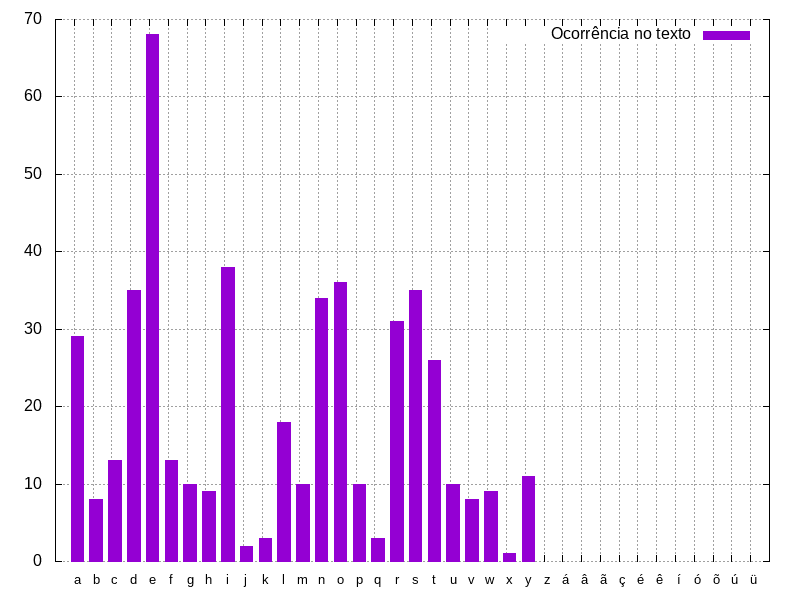
\includegraphics[width=0.8\linewidth]{freq-en.png}
    \captionof{figure}{Histograma do texto em inglês}
\end{center}\vspace{1cm}

\begin{center}\vspace{1cm}
    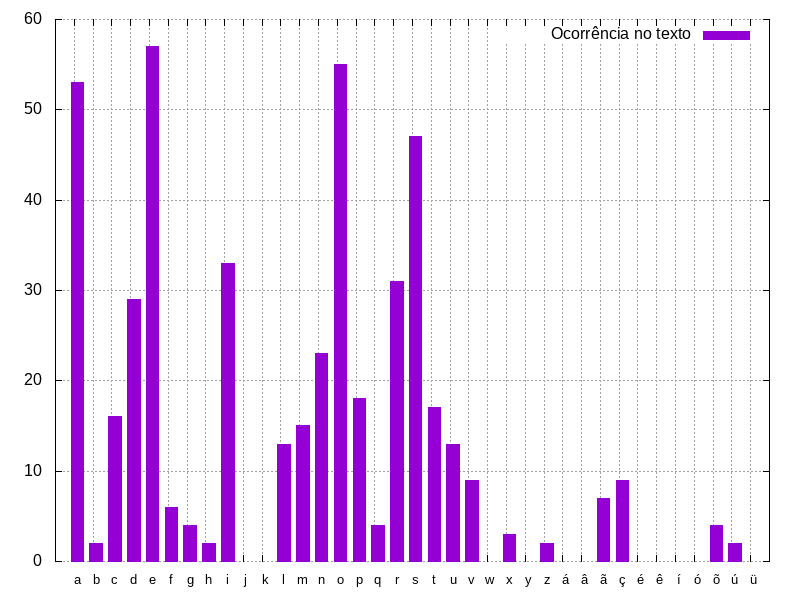
\includegraphics[width=0.8\linewidth]{freq-ptbr.png}
    \captionof{figure}{Histograma do texto em português}
\end{center}\vspace{1cm}

\section*{Método de classificação}
Pela análise do nosso problema, consideramos utilizar \textbf{modelos preditivos} para poder classificar o texto com base em outros textos de entrada previamente classificados.

\subsection*{Modelo baseado em distância}
A técnica que decidimos utilizar é baseado na \textbf{distância euclidiana}~\ref{eqn:euclid} entre o texto sem classificação e os textos da base de conhecimento. Como a distância envolvendo a quantidade de ocorrência poderia dar uma falsa informação, usamos a porcentagem que cada letra é encontrada no texto.

\vspace{0.5cm}
\begin{equation}
d(x_i, x_j) = \sqrt{\sum_{l=1}^{d} (x^l_i - x^l_j)^2}
\label{eqn:euclid}
\end{equation}\vspace{0.5cm}

Como a distância para o mais próximo pode não ser tão precisa, a utilização do algoritmo \emph{k-NN}, do inglês \emph{k-Nearest Neighbor} se fez necessária, assim calculamos a distância para cada texto e fazemos uma média dos \emph{n} primeros.

\begin{center}\vspace{1cm}
    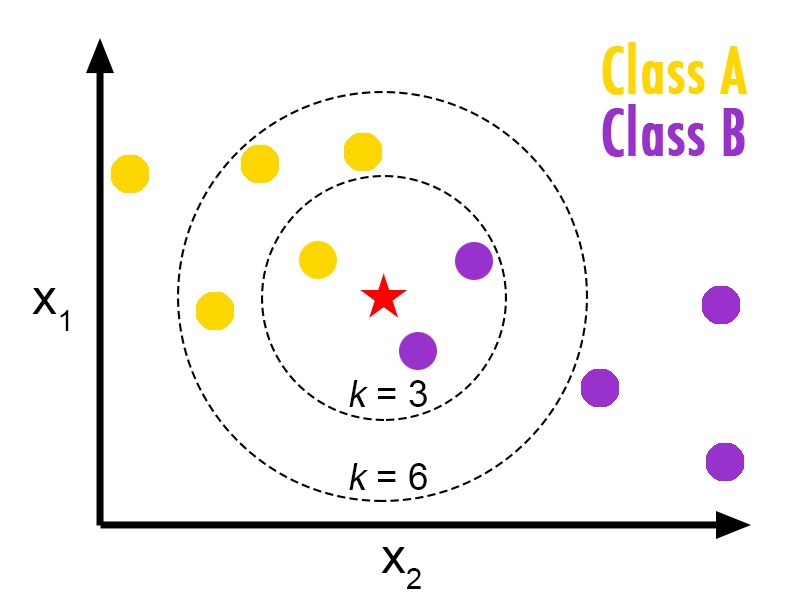
\includegraphics[width=0.5\linewidth]{knn.png}
    \captionof{figure}{Representação do \emph{k-NN} (Fonte: Medium~\cite{site:knn})}
\end{center}\vspace{1cm}

\section*{Conclusão}
Sabemos que o método que escolhemos para a identificação pode ser um pouco custoso para uma base de dados muito grande, mas a predição que fazemos é importante para casos em que se utiliza redes neurais ou outras teorias mais avançadas de Inteligência Artificial. Assim, temos uma idéia da potencialização que algoritmos baseados em \emph{Machine Learning} fornecem para um projeto, maximizando a eficiência e a velocidade em que diversos algoritmos são executados.
\nocite{*}
\bibliographystyle{plain} % Plain referencing style
\bibliography{poster} % Use the example bibliography file sample.bib

\end{multicols}
\end{document}